\section{배경지식 및 위협 모델}

\subsection{공격자 능력 모델}

% 본 연구가 상정하는 공격자는 (a) MAVLink 엔드포인트(직렬 포트, UDP/TCP 링크, 경로상 relay)에 도달할 수 있고, (b) 신뢰 sysid를 사칭하거나 rogue sysid로 잘 정형된(well-formed) 프레임을 주입할 수 있으며, (c) GNSS/센서 경계에서 완만한 스푸핑 신호를 부과할 수 있고, (d) 공유 상향링크 대역을 포화시킬 수 있다. 공격자는 회피(evasion) 튜닝이나 운용자 기만을 사용하지 않는다 --- 위협과 그 탐지 가능성을 동시에 실증하는 것이 목적이므로, 모든 주입 프레임은 공격자의 실제 헤더로 평문 전송된다. 실제 군용 위성 RF 신호를 복조하거나 암호 장비를 탈취하는 강한 공격자는 가정하지 않는다.

% 전통적인 적대적 머신러닝 문헌의 white-box/gray-box/black-box 구분\cite{nist_aml}을 적용하면, 본 연구의 프로토콜/링크 계층 공격자는 대체로 gray-box/black-box이다 --- 네트워크 상에서 패킷을 관찰·재전송·위조하는 것만으로 공격이 성립하며 대상의 내부 소프트웨어 구조를 알 필요가 없다. 반면 GPS/센서 스푸핑은 EKF 융합 구조에 대한 이해가 성공률을 높인다는 점에서 gray-box에 가깝고, AI 에이전트 계층(7장)에 대한 공격은 이 스펙트럼의 확장으로 위치지을 수 있다.
본 연구에서 상정하는 공격자는 네 가지 능력을 갖는다. 
%
첫째, 공격자는 MAVLink 엔드포인트에 도달할 수 있다. 
%
여기서 엔드포인트는 직렬 포트, UDP/TCP 링크, 또는 경로상 relay를 포함한다. 
%
둘째, 공격자는 신뢰 sysid를 사칭하거나 rogue sysid로 잘 정형된 MAVLink 프레임을 주입할 수 있다. 
%
셋째, 공격자는 GNSS 또는 센서 경계에서 완만한 스푸핑 신호를 부과할 수 있다. 
%
넷째, 공격자는 공유 상향링크 대역을 포화시킬 수 있다.
%
반대로 더 강한 공격자는 가정하지 않는다. 공격자는 실제 군용 위성 RF 신호를 복조하지 않고, 암호 장비를 탈취하지 않으며, 실제 GNSS 신호를 송신하지 않는다. 또한 회피 (evasion) 튜닝이나 운용자 기만을 사용하지 않는다. 이 연구의 목적은 위협과 탐지 가능성을 동시에 실증하는 것이므로, 모든 주입 프레임은 공격자가 설정한 실제 헤더로 평문 전송된다. 신규 탐지불가 공격의 발명이나 운용자 화면 위조도 연구 범위에 포함하지 않는다.
%
전통적인 적대적 머신러닝 문헌의 화이트박스 (white-box), 그레이박스 (gray-box), 블랙박스 (black-box) 구분~\cite{nist_aml}을 적용하면, 본 연구의 프로토콜 및 링크 계층 공격자는 대체로 그레이박스 또는 블랙박스에 해당한다. 
%
네트워크 상에서 패킷을 관찰, 재전송, 위조할 수 있으면 공격이 성립하며, 대상의 내부 소프트웨어 구조를 알 필요는 없다. 
%
반면 GPS 및 센서 스푸핑은 EKF 융합 구조에 대한 이해가 성공률을 높일 수 있으므로 gray-box에 가깝다. 
%
AI 에이전트 계층 공격은 이 지식 수준 스펙트럼의 확장으로 위치지을 수 있으며, 7장에서 RED/BLUE 정보 격리와 도구 경계 설계를 통해 다룬다.

% \subsection{공격 구현의 세 계층}

% 14개 공격은 세 계층의 주입 메커니즘으로 구현된다.

% \begin{itemize}[leftmargin=*]
%     \item \textbf{MAVLink 프레임 위조(제어 계층).} \texttt{rc\_override.py}, \texttt{command\_injection.py}, \texttt{replay.py}, \texttt{mission\_tamper.py}, \texttt{param\_tamper.py}, \texttt{mav\_flood.py}가 열려 있는 \texttt{pymavlink} 연결을 통해 위조 프레임을 링크에 올린다. 연결의 \texttt{source\_system}/\texttt{source\_component}가 곧 피해 기체가 보는 헤더이므로, 신뢰 sysid 사칭과 rogue sysid 주입을 동일 코드로 구현한다. MAVLink는 v1은 물론 v2에서도 메시지 서명이 선택 사항이라 평문 전송되는 경우가 많다는 사실이 이 계층 전체의 구조적 취약점이다\cite{uas_survey_sok,mavlink_nutshell,cve202010283}.
%     \item \textbf{센서/GNSS 경계 주입(항법 계층).} \texttt{gps\_spoof.py}, \texttt{gnss\_jam.py}, \texttt{sensor\_spoof.py}(지자기), \texttt{imu\_spoof.py}, \texttt{baro\_spoof.py}가 ArduPilot SITL이 EKF에 값을 발행하기 직전의 센서 백엔드 파라미터(\texttt{SIM\_GPS1\_GLTCH\_*}, \texttt{SIM\_MAG1\_OFS}, \texttt{SIM\_ACC*\_BIAS}, \texttt{SIM\_BARO\_GLITCH} 등)를 램프시켜, RF/nav 계층의 스푸퍼를 센서 경계에서 모델링한다. GPS 기만의 핵심은 급격한 점프가 아니라 저속 walk-off로, EKF innovation 게이팅을 넘지 않도록 초당 1 m씩 오프셋을 성장시켜 추정기가 위조된 위치를 계속 융합하게 만든다.
%     \item \textbf{경로상 링크 조작(전송 계층).} \texttt{mav\_proxy.py}(userspace MITM relay) + \texttt{link\_shaper.py}(큐 지연·지터·손실) + \texttt{mav\_flood.py}(대역 포화)가 bent-pipe SATCOM의 고지연·고손실·공유 대역 특성을 userspace에서 에뮬레이션한다\cite{theaterq}.
% \end{itemize}

\subsection{공격 구현의 세 계층}
14개 공격은 세 계층의 주입 메커니즘으로 구현한다. 
%
세 계층은 MAVLink 프레임 위조를 다루는 제어 계층, GNSS 및 센서 경계 주입을 다루는 항법 계층, 경로상 링크 조작을 다루는 전송 계층이다.
%
\begin{itemize}[leftmargin=*]
    \item \textbf{MAVLink 프레임 위조 (제어 계층).}
    \texttt{rc\_override.py},~\texttt{command\_injection.py},~\texttt{mission\_tamper.py}, ~\texttt{param\_tamper.py},~\texttt{replay.py},~\texttt{mav\_flood.py}는 열린~\texttt{pymavlink} 연결을 통해 위조 프레임을 링크에 주입한다. 연결의~\texttt{source\_system}과~\texttt{source\_component}는 대상 기체가 관측하는 헤더가 되므로, 신뢰 sysid 사칭과 rogue sysid 주입을 동일 코드 경로로 구현한다. MAVLink v1은 물론 MAVLink v2에서도 메시지 서명이 선택 기능에 머물며, 서명을 활성화하지 않는 구성에서는 평문 메시지 주입이 가능하다는 점이 이 계층의 구조적 취약점이다~\cite{uas_survey_sok,mavlink_nutshell,cve202010283}.
    \item \textbf{센서/GNSS 경계 주입 (항법 계층).}
    ~~\texttt{gps\_spoof.py},~\texttt{gnss\_jam.py},~\texttt{sensor\_spoof.py}, ~\texttt{imu\_spoof.py},   
    ~\texttt{baro\_spoof.py}는 ArduPilot SITL이 EKF에 값을 발행하기 직전의 센서 백엔드 파라미터를 점진적으로 변화시킨다. 사용 파라미터는~\texttt{SIM\_GPS1\_GLTCH\_*},~\texttt{SIM\_MAG1\_OFS}, ~\texttt{SIM\_ACC*\_BIAS},~\texttt{SIM\_BARO\_GLITCH} 등을 포함한다. 이 방식은 실제 RF 또는 물리 센서 공격을 수행하지 않고, RF/navigation 계층 스푸퍼의 효과를 센서 경계에서 모델링한다. GPS 기만의 핵심은 급격한 점프가 아니라 저속 walk-off이다. 본 연구는 EKF innovation 게이팅을 넘지 않도록 초당 1 m 수준으로 오프셋을 증가시켜 추정기가 위조 위치를 계속 융합하는 조건을 만든다.
    \item \textbf{경로상 링크 조작 (전송 계층).}
    \texttt{mav\_proxy.py},~\texttt{link\_shaper.py},~\texttt{mav\_flood.py}는 각각 사용자 공간 MITM relay, 큐 지연·지터·손실 shaper, 대역 포화 flooder로 동작한다. 이 조합은 bent-pipe SATCOM에서 나타나는 고지연, 고손실, 공유 대역 특성을 사용자 공간에서 에뮬레이션한다~\cite{theaterq}. 이 계층은 실제 위성, 실제 RF 송수신, 루트 권한, kernel-level \texttt{netem} 없이 BLOS C2 링크 열화와 DoS 조건을 재현한다.
\end{itemize}

\subsection{관련 프로토콜·플랫폼 계층 문헌}

% \subsubsection{MAVLink 계층}
% MAVLink는 GCS와 UxV 사이의 사실상 표준 통신 프로토콜이나, v1과 v2 모두 기본적으로 평문 전송을 사용하고 메시지 서명은 선택적 기능에 그친다\cite{uas_survey_sok,mavlink_nutshell}. 이로 인해 명령 주입을 통한 비행 모드/임무 조작, 과거 패킷 재사용 재전송, 웨이포인트 변조, 제어 안정성 저하 파라미터 남용 공격이 실증적으로 보고되어 왔다\cite{ficco2022mavlink,mavshield,ardupilot_reverse,muvids,mavlink_survey_threats,mavlink_vuln_sciup}. 최근에는 세션 타입(session type) 이론을 이용해 MAVLink 메시지 시퀀스를 정형적으로 검증하려는 시도도 제안되었다\cite{session_types_mavlink}.

% \subsubsection{로봇 미들웨어 및 인접 플랫폼}
% UGV 등 지상 이동체의 상위 자율주행 스택이 ROS~2/DDS로 구성되는 경우, SROS~2가 인증서 기반 인증·권한 관리를 제공함에도 keystore 유출이나 QoS 정책 동기화 결함으로 topic spoofing이 가능함이 보고되었다\cite{ros2_supply_chain,sros2_insecurity,ros2_threat_model,ros2_lidar_spoofing}. 본 연구의 실제 구현 범위(5~8장)는 MAVLink 제어 계층·센서/GNSS 경계·위성/BLOS 링크에 한정되며, ROS~2/DDS 계층은 인접 플랫폼의 문헌 조사로만 다룬다. 쿼드러페드·휴머노이드와 같은 인접 자율 플랫폼의 위협 지형 역시 유사한 인증 부재 문제를 공유한다\cite{quadruped_survey,humanoid_sok}.

% \subsubsection{시뮬레이션 및 공격 재현 플랫폼}
% ArduPilot SITL은 실제 하드웨어 없이 UAV/UGV의 비행/주행 제어 로직을 그대로 구동할 수 있어 공격·방어 실험에 널리 사용되어 왔다. UAVLnQ는 ArduPilot SITL과 ns-3 네트워크 시뮬레이터를 ZMQ 미들웨어로 동기화하여 명령 주입·스푸핑·서비스 거부 공격을 군집 시나리오에서 재현하는 플랫폼을 제공하며\cite{uavlnq}, MIXED-SENSE는 실제와 유사한 센서 인식을 결합한 UAV 사이버보안 테스트베드를 제안하였다\cite{mixed_sense}. 위성/BLOS 링크의 지연·지터·손실 재현에는 \texttt{tc/netem} 기반 접근이 문헌상 널리 쓰이나\cite{theaterq}, 본 연구는 root/kernel 권한이 필요한 \texttt{netem} 대신 userspace MITM MAVLink relay 기반 shaper/flooder로 동일한 링크 특성을 재현한다(5.5절, \texttt{src/attacks/mav\_proxy.py}). 본 연구는 이러한 선행 테스트베드의 구성 원칙 --- SITL 기반 제어 재현성, 네트워크 계층 공격 주입 가능성 --- 을 계승하되, 여기에 실제 LLM 기반 RED/BLUE 에이전트 계층(7장)을 추가로 결합한다.

\subsubsection{MAVLink 계층}

MAVLink는 GCS와 UxV 사이의 사실상 표준 통신 프로토콜이다. 그러나 v1과 v2 모두 기본적으로 평문 전송을 사용하며, 메시지 서명은 선택적 기능에 머문다~\cite{uas_survey_sok,mavlink_nutshell}. 기존 연구는 명령 주입을 통한 비행 모드 또는 임무 조작, 과거 패킷 재사용을 통한 재전송, 웨이포인트 변조, 제어 안정성을 저해하는 파라미터 남용 공격을 보고한다~\cite{ficco2022mavlink,mavshield,ardupilot_reverse,muvids,mavlink_survey_threats,mavlink_vuln_sciup}. 최근 연구는 세션 타입 (Session type) 이론을 이용하여 MAVLink 메시지 시퀀스를 정형적으로 검증하는 접근도 제안한다~\cite{session_types_mavlink}.

\subsubsection{로봇 미들웨어 및 인접 플랫폼}

UGV 등 지상 이동체의 상위 자율주행 스택이 ROS~2/DDS로 구성되는 경우, SROS~2는 인증서 기반 인증과 권한 관리를 제공한다. 그러나 관련 연구는 keystore 유출이나 QoS 정책 동기화 결함으로 topic spoofing이 가능함을 보고한다~\cite{ros2_supply_chain,sros2_insecurity,ros2_threat_model,ros2_lidar_spoofing}. 본 연구의 실제 구현 범위는 MAVLink 제어 계층, 센서/GNSS 경계, 위성/BLOS 링크에 한정한다. ROS~2/DDS 계층은 인접 플랫폼의 문헌 배경으로만 다룬다. 쿼드러페드와 휴머노이드 같은 인접 자율 플랫폼도 인증 부재, 센서 신뢰성, 원격 명령 경로 보호 문제를 공유한다~\cite{quadruped_survey,humanoid_sok}.

\subsubsection{시뮬레이션 및 공격 재현 플랫폼}

ArduPilot SITL은 실제 하드웨어 없이 UAV와 UGV의 비행 및 주행 제어 로직을 실행할 수 있어 공격·방어 실험에 널리 쓰인다. UAVLnQ는 ArduPilot SITL과 ns-3 네트워크 시뮬레이터를 ZMQ 미들웨어로 동기화하여 명령 주입, 스푸핑, 서비스 거부 공격을 군집 시나리오에서 재현하는 플랫폼을 제공한다~\cite{uavlnq}. MIXED-SENSE는 실제와 유사한 센서 인식을 결합한 UAV 사이버보안 테스트베드를 제안한다~\cite{mixed_sense}. 위성/BLOS 링크의 지연, 지터, 손실 재현에는 \texttt{tc/netem} 기반 접근이 문헌상 널리 쓰인다~\cite{theaterq}. 본 연구는 루트 및 커널 권한이 필요한 \texttt{netem} 대신 사용자 공간 MITM MAVLink relay 기반 shaper/flooder로 동일한 링크 특성을 재현한다. 따라서 선행 테스트베드의 SITL 기반 제어 재현성과 네트워크 계층 공격 주입 가능성을 계승하면서, 실제 LLM 기반 RED/BLUE 에이전트 계층을 추가로 결합한다.

\subsection{공격 표면 개요}

% \begin{figure}[t!]
% \centering
% 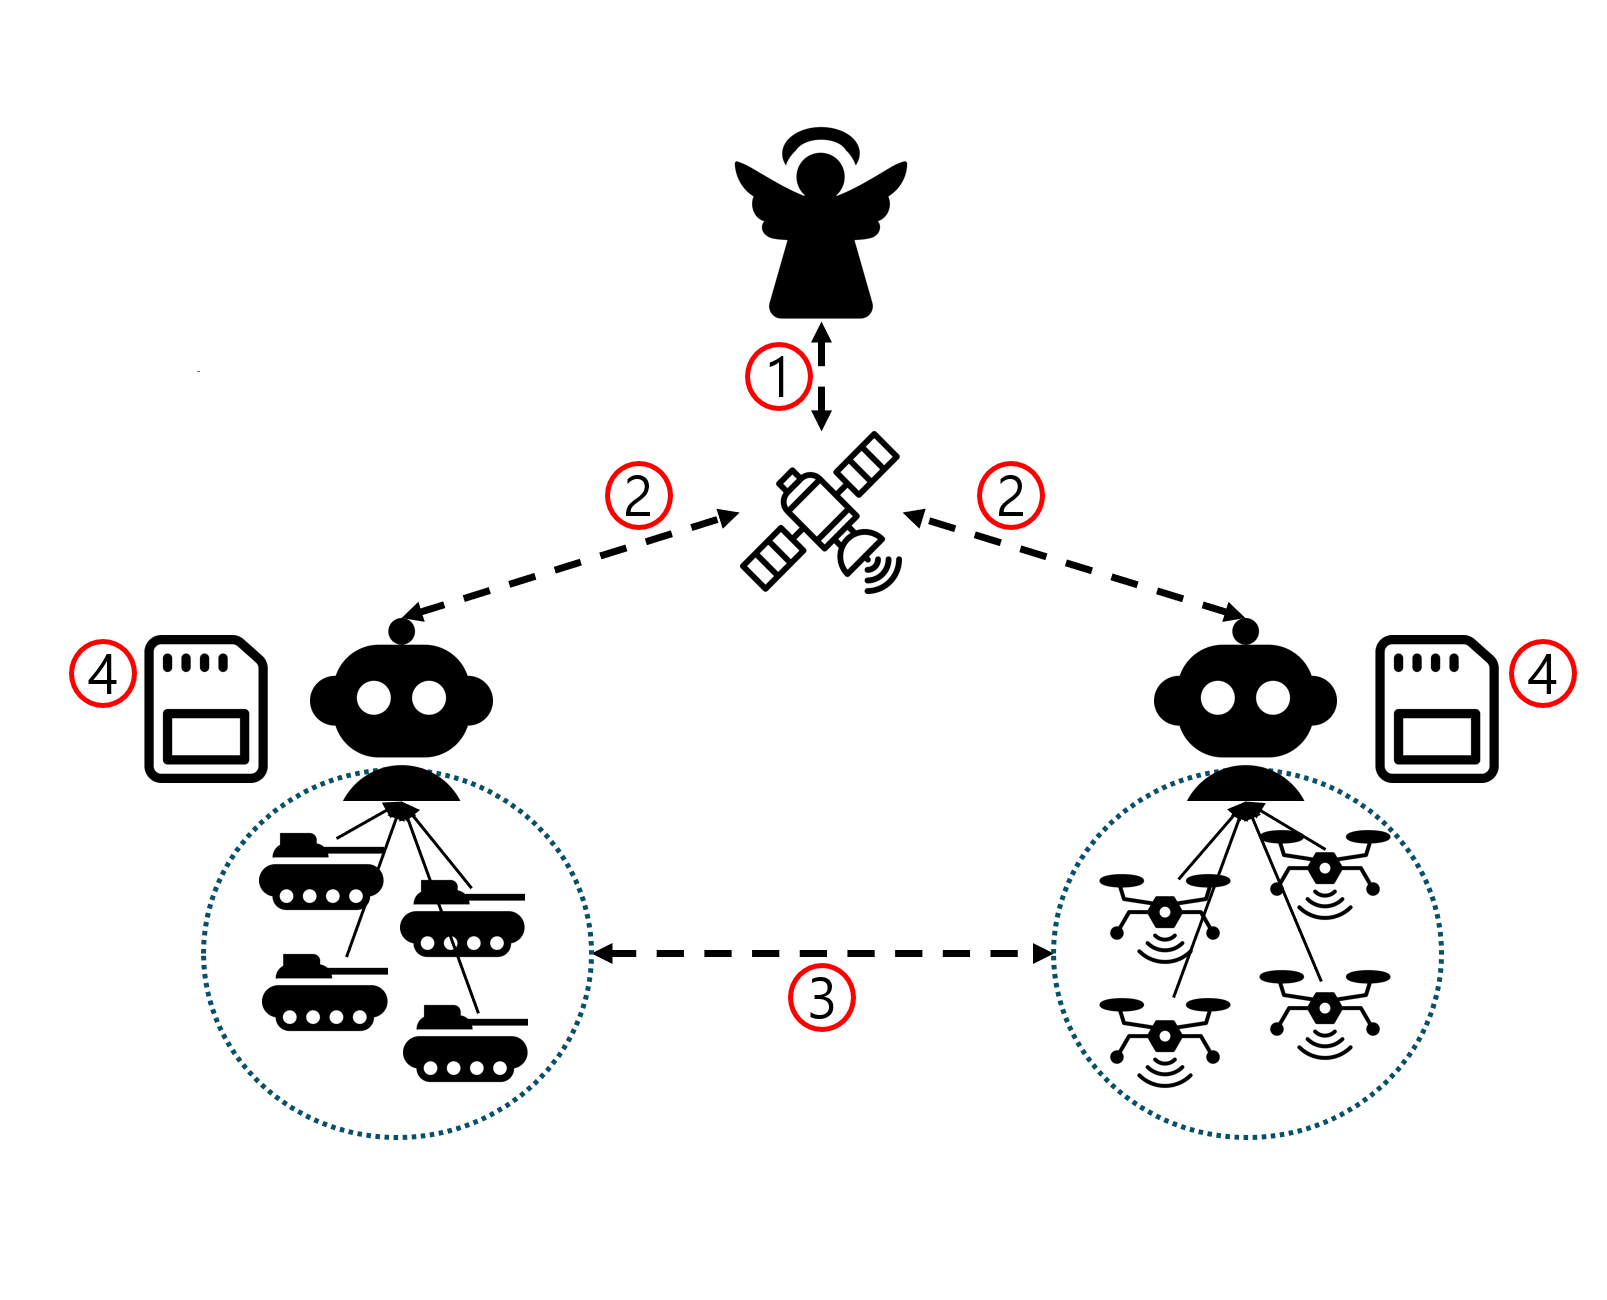
\includegraphics[width=0.85\textwidth]{content/figures/attack_surface.png}
% \caption{다계층 무인체계의 공격 표면(attack surface) 개요. C2/GCS로부터 위성/무선 링크를 거쳐 UGV·UAV로 이어지는 통신 경로와, 각 에이전트가 참조하는 로컬 저장소를 함께 나타낸다. 번호는 본문에서 설명하는 네 가지 공격 지점(①--④)에 대응하며, ①·②는 5장에서 실제로 구현·실측한 MAVLink/링크 계층 공격 지점, ③·④는 7장의 AI 에이전트 아키텍처(RED/BLUE 정보 격리, 지휘관 로컬 상태)와 개념적으로 대응한다.}
% \label{fig:attack_surface}
% \end{figure}

% 표~\ref{tab:attack_defense_overview}는 5~6장에서 상술할 14개 공격(+ADS-B 탐지기 전용 시나리오)과 그 대응 방어를 도메인별로 요약한 것이다. 각 공격은 \texttt{src/attacks/}, 각 방어는 \texttt{src/defenses/} 아래의 실제 파이썬 모듈로 존재한다.

% \begin{table}[t!]
% \centering
% \caption{도메인별 공격/방어 개요 --- 구현 및 실측 완료 (구현: \texttt{src/attacks/}, \texttt{src/defenses/})}
% \label{tab:attack_defense_overview}
% \renewcommand{\arraystretch}{1.2}
% \scriptsize
% \begin{adjustbox}{width=\textwidth}
% \begin{tabular}{p{1.3cm} p{3.4cm} p{3.5cm} p{3.0cm} p{2.6cm}}
% \toprule
% \textbf{도메인} & \textbf{공격} & \textbf{공격 모듈} & \textbf{방어 모듈} & \textbf{예방 티어} \\
% \midrule
% UAV & RC 오버라이드(PITCH ch2) & \texttt{rc\_override.py} & D5 + D6 & [LIVE] BRAKE \\
% UAV & 명령 주입(DO\_SET\_MODE$\to$RTL) & \texttt{command\_injection.py} & D2 + D-SIGN & [SIGN] \\
% UAV & GPS 완만 기만 & \texttt{gps\_spoof.py} & D3 & [LIVE] EKF 소스전환 \\
% UAV & GNSS 재밍/거부 & \texttt{gnss\_jam.py} & D7(GNSS 건전성) & [DETECT-ONLY]+[NATIVE-FS] \\
% UAV & 지자기 스푸핑 & \texttt{sensor\_spoof.py} & D-XCHK & [DETECT-ONLY] \\
% UAV & IMU / 기압 스푸핑 & \texttt{imu\_spoof.py}, \texttt{baro\_spoof.py} & D-IMU, D-BARO & [DETECT-ONLY] \\
% UAV & 미션 / 파라미터 변조 & \texttt{mission\_tamper.py}, \texttt{param\_tamper.py} & D-MISSION, D-PARAM + D-SIGN & [SIGN]+[LIVE-restore] \\
% UAV & ADS-B 유령 항공기 & (하니스 주입) & D-ADSB & [DETECT-ONLY] \\
% \hdashline
% UGV & 조향 채널 오버라이드 & \texttt{rover\_steering.py} & D5 + D6 & [LIVE] HOLD \\
% UGV & 명령 주입 + 이동 중 disarm & \texttt{command\_injection.py} & D2 + D-SIGN & [SIGN] \\
% UGV & GPS 완만 기만 & \texttt{gps\_spoof.py} & D3 & [LIVE] EKF 소스전환 \\
% \hdashline
% 위성/BLOS & 링크 열화(지연/지터/손실) & \texttt{mav\_proxy.py}+\texttt{link\_shaper.py} & D4 & [NATIVE-FS-ready] \\
% 위성/BLOS & DoS 블랙아웃 & \texttt{mav\_proxy.py} & D4 & [NATIVE-FS-ready] \\
% 위성/BLOS & 대역폭 flooding & \texttt{mav\_flood.py} & D4(ingress-rate) & [LIVE] rate-limit \\
% 위성/BLOS & 프레임 재전송(replay) & \texttt{replay.py} & D-REPLAY + D-SIGN & [SIGN] \\
% \bottomrule
% \end{tabular}
% \end{adjustbox}
% \end{table}

% 각 행의 상세 위협 서사·창발 결과·증거 경로는 5장에서, 탐지·차단·복구의 결합 논리와 정직성 티어 태깅은 6장에서, 이 파이프라인을 실제로 구동하는 LLM 기반 RED/BLUE 에이전트 아키텍처는 7장에서 다룬다.

그림~\ref{fig:attack_surface}은 본 연구에서 다루는 다계층 무인체계 공격 표면을 나타낸다. C2/GCS로부터 위성 또는 무선 링크를 거쳐 UGV와 UAV로 이어지는 통신 경로가 핵심 공격면을 구성한다. 또한 각 에이전트가 참조하는 로컬 저장소와 지휘관 상태도 별도의 신뢰 경계로 다룬다.

\begin{figure}[t!]
\centering
% \includegraphics[width=0.85\textwidth]{content/figures/agent_surface.png}
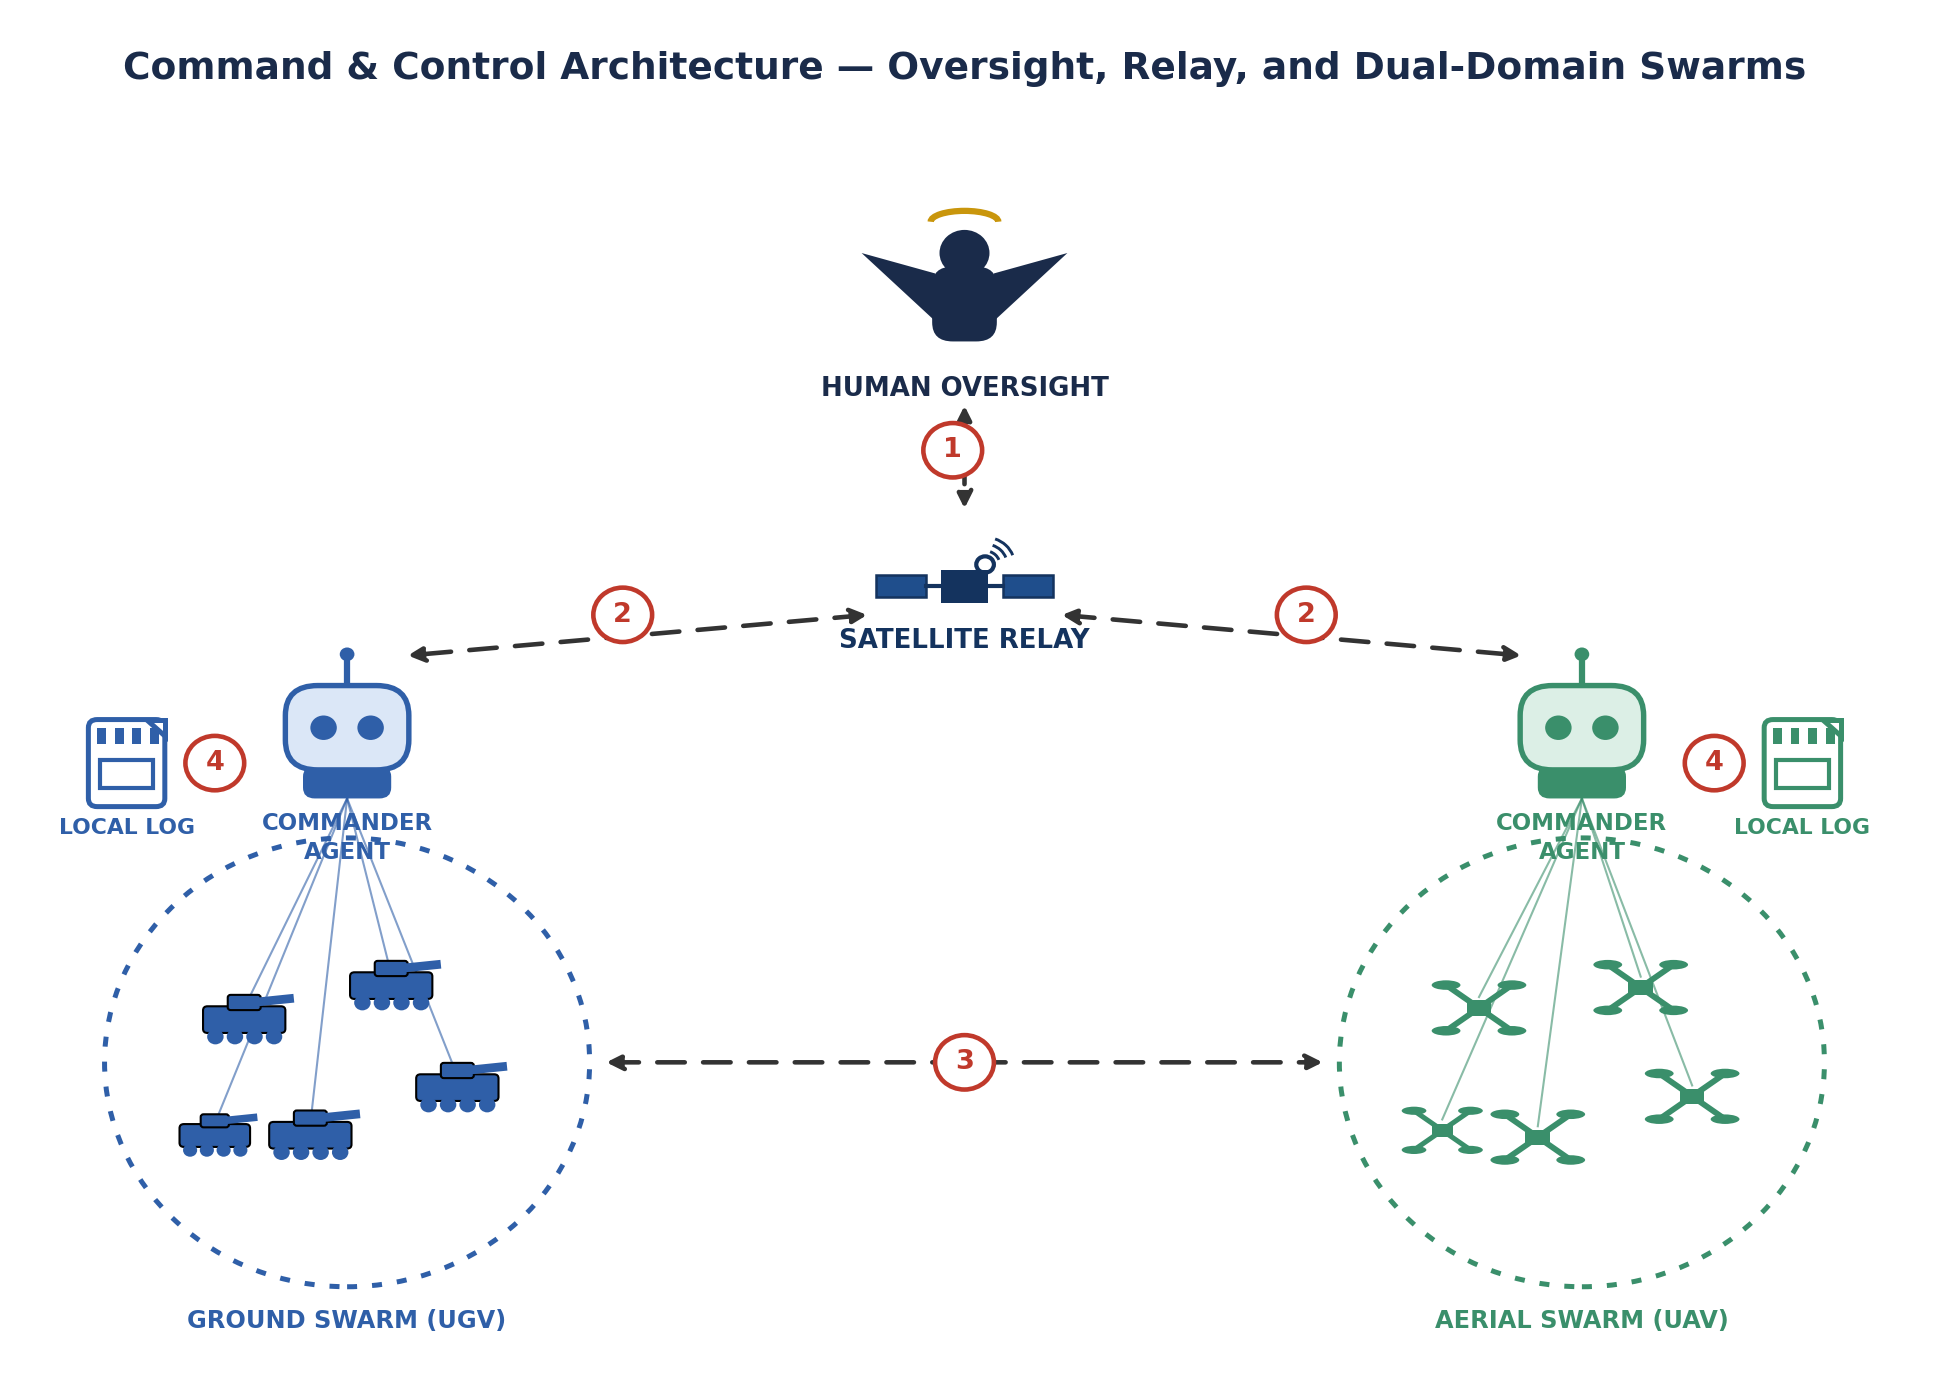
\includegraphics[width=0.75\textwidth]{content/figures/command_control_diagram.png}
\caption{다계층 무인체계의 공격 표면 (Attack surface) 개요. C2/GCS로부터 위성/무선 링크를 거쳐 UGV·UAV로 이어지는 통신 경로와, 각 에이전트가 참조하는 로컬 저장소를 함께 나타낸다. 번호는 본문에서 설명하는 네 가지 공격 지점 (①--④)에 대응한다. ①·②는 5장에서 구현·실측하는 MAVLink/링크 계층 공격 지점이며, ③·④는 7장의 AI 에이전트 아키텍처, RED/BLUE 정보 격리, 지휘관 로컬 상태와 개념적으로 대응한다.}
\label{fig:attack_surface}
\end{figure}

표~\ref{tab:attack_defense_overview}는 5장과 6장에서 상세히 다루는 14개 공격 및 ADS-B 탐지기 전용 시나리오와 그 대응 방어를 도메인별로 요약한다. 각 공격은 \texttt{src/attacks/}, 각 방어는 \texttt{src/defenses/} 아래의 실제 파이썬 모듈로 존재한다.

\begin{table}[t!]
\centering
\caption{도메인별 공격/방어 개요 --- 구현 및 실측 대상}
\label{tab:attack_defense_overview}
\renewcommand{\arraystretch}{1.2}
\scriptsize
\begin{adjustbox}{width=\textwidth}
\begin{tabular}{p{1.3cm} p{3.4cm} p{3.5cm} p{3.0cm} p{2.6cm}}
\toprule
\textbf{도메인} & \textbf{공격} & \textbf{공격 모듈} & \textbf{방어 모듈} & \textbf{예방 티어} \\
\midrule
UAV & RC 오버라이드(PITCH ch2) & \texttt{rc\_override.py} & D5 + D6 & [LIVE] BRAKE \\
UAV & 명령 주입(DO\_SET\_MODE$\to$RTL) & \texttt{command\_injection.py} & D2 + D-SIGN & [SIGN] \\
UAV & GPS 완만 기만 & \texttt{gps\_spoof.py} & D3 & [LIVE] EKF 소스전환 \\
UAV & GNSS 재밍/거부 & \texttt{gnss\_jam.py} & D7 (GNSS 건전성) & [DETECT-ONLY]+[NATIVE-FS] \\
UAV & 지자기 스푸핑 & \texttt{sensor\_spoof.py} & D-XCHK & [DETECT-ONLY] \\
UAV & IMU / 기압 스푸핑 & \texttt{imu\_spoof.py}, \texttt{baro\_spoof.py} & D-IMU, D-BARO & [DETECT-ONLY] \\
UAV & 미션 / 파라미터 변조 & \texttt{mission\_tamper.py}, \texttt{param\_tamper.py} & D-MISSION, D-PARAM + D-SIGN & [SIGN]+[LIVE-restore] \\
UAV & ADS-B 유령 항공기 & 하니스 주입 & D-ADSB & [DETECT-ONLY] \\
\hdashline
UGV & 조향 채널 오버라이드 & \texttt{rover\_steering.py} & D5 + D6 & [LIVE] HOLD \\
UGV & 명령 주입 + 이동 중 disarm & \texttt{command\_injection.py} & D2 + D-SIGN & [SIGN] \\
UGV & GPS 완만 기만 & \texttt{gps\_spoof.py} & D3 & [LIVE] EKF 소스전환 \\
\hdashline
위성/BLOS & 링크 열화 (지연/지터/손실) & \texttt{mav\_proxy.py}+\texttt{link\_shaper.py} & D4 & [NATIVE-FS-ready] \\
위성/BLOS & DoS 블랙아웃 & \texttt{mav\_proxy.py} & D4 & [NATIVE-FS-ready] \\
위성/BLOS & 대역폭 flooding & \texttt{mav\_flood.py} & D4(ingress-rate) & [LIVE] rate-limit \\
위성/BLOS & 프레임 재전송(replay) & \texttt{replay.py} & D-REPLAY + D-SIGN & [SIGN] \\
\bottomrule
\end{tabular}
\end{adjustbox}
\end{table}

각 행의 상세 위협 서사, 창발 결과, 증거 경로는 5장에서 다룬다. 탐지, 차단, 복구의 결합 논리와 정직성 티어 태깅은 6장에서 다룬다. 이 파이프라인을 구동하는 LLM 기반 RED/BLUE 에이전트 아키텍처는 7장에서 다룬다.